%\documentclass{book}
%
%\usepackage{fancyhdr}
%\usepackage{extramarks}
%\usepackage{amsmath}
%\usepackage{amsthm}
%\usepackage{amsfonts}
%\usepackage{tikz}
%\usepackage{enumerate}
%\usepackage{graphicx}
%\graphicspath{ {images/} }
%\usepackage[plain]{algorithm}
%\usepackage{algpseudocode}
%\usepackage[document]{ragged2e}
%\usepackage{textcomp}
%\usepackage{color}   %May be necessary if you want to color links
%\usepackage{import}
%\usepackage{natbib}
%\usepackage{hyperref}
%\hypersetup{
%    colorlinks=true, %set true if you want colored links
%    linktoc=all,     %set to all if you want both sections and subsections linked
%    linkcolor=black,  %choose some color if you want links to stand out
%}
%
%\usetikzlibrary{automata,positioning}
%
%
%% Basic Document Settings
%
%
%\topmargin=-0.45in
%\evensidemargin=0in
%\oddsidemargin=0in
%\textwidth=6.5in
%\textheight=9.0in
%\headsep=0.25in
%\setlength{\parskip}{1em}
%
%\linespread{1.1}
%
%\pagestyle{fancy}
%\lhead{\hmwkAuthorName}
%\lfoot{\lastxmark}
%\cfoot{\thepage}
%
%\renewcommand\headrulewidth{0.4pt}
%\renewcommand\footrulewidth{0.4pt}
%
%\setlength\parindent{0pt}
%
%
%\newcommand{\hmwkTitle}{Math Review Notes---Abstract Algebra}
%\newcommand{\hmwkAuthorName}{\textbf{G. Faletto} }
%
%
%%%%%% Title Page
%
%
%\title{
%    \vspace{2in}
%    \textmd{\textbf{ \hmwkTitle}}\\
%}
%
%\author{Gregory Faletto}
%\date{}
%
%\renewcommand{\part}[1]{\textbf{\large Part \Alph{partCounter}}\stepcounter{partCounter}\\}
%
%
%%%%%% Various Helper Commands
%
%
%%%%%% Useful for algorithms
%\newcommand{\alg}[1]{\textsc{\bfseries \footnotesize #1}}
%
%%%%%% For derivatives
%\newcommand{\deriv}[2]{\frac{\mathrm{d} #1}{\mathrm{d} #2}}
%
%%%%%% For partial derivatives
%\newcommand{\pderiv}[2]{\frac{\partial #1}{\partial #2}}
%
%%%%%% Integral dx
%\newcommand{\dx}{\mathrm{d}x}
%
%%%%%% Alias for the Solution section header
%\newcommand{\solution}{\textbf{\large Solution}}
%
%%%%%% Probability commands: Expectation, Variance, Covariance, Bias
%\newcommand{\E}{\mathbb{E}}
%\newcommand{\Var}{\mathrm{Var}}
%\newcommand{\Cov}{\mathrm{Cov}}
%\newcommand{\Bias}{\mathrm{Bias}}
%\newcommand\indep{\protect\mathpalette{\protect\independenT}{\perp}}
%\def\independenT#1#2{\mathrel{\rlap{$#1#2$}\mkern2mu{#1#2}}}
%\DeclareMathOperator{\Tr}{Tr}
%
%\theoremstyle{definition}
%\newtheorem{theorem}{Theorem}
%\theoremstyle{definition}
%\newtheorem{proposition}[theorem]{Proposition}
%\theoremstyle{definition}
%\newtheorem{lemma}[theorem]{Lemma}
%\theoremstyle{definition}
%\newtheorem{corollary}{Corollary}[theorem]
%\theoremstyle{definition}
%\newtheorem{definition}{Definition}[section]
%\newtheorem{remark}{Remark}
%\theoremstyle{definition}
%\newtheorem{exercise}{Exercise}
%\theoremstyle{definition}
%\newtheorem{example}{Example}[section]
%
%%%%%% Tilde
%\newcommand{\textapprox}{\raisebox{0.5ex}{\texttildelow}}
%
%\begin{document}
%
%\maketitle
%
%\pagebreak
%
%\tableofcontents
%
%\
%
%\
%
%\begin{center}
%Last updated \today
%\end{center}
%
%
%
%\newpage
%
%%
%%
%%
%%
%%
%%
%%
%%
%%%
%% Abstract Algebra

\chapter{Abstract Algebra}

These are my notes from reading \textit{Elementary Abstract Algebra} by W. Edwin Clark, available for free download on his website: \url{http://shell.cas.usf.edu/~wclark/#ELEMENTARY_ABSTRACT_ALGEBRA}

% Chapter 1
\section{Chapter 1: Binary Operations}

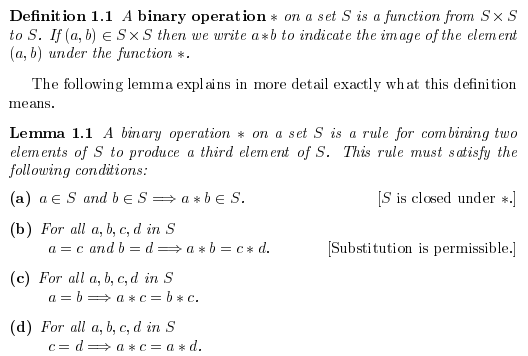
\includegraphics[scale=0.65]{binary_operation}

%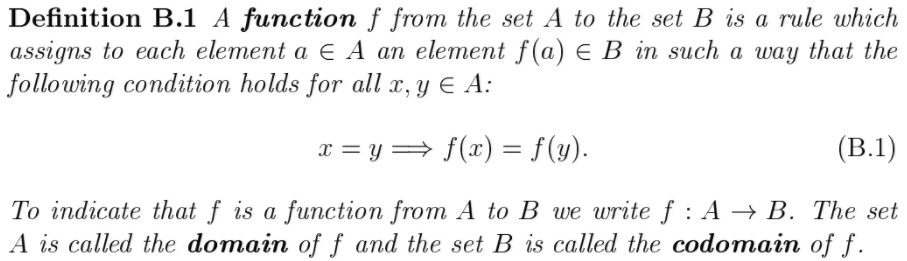
\includegraphics[scale=0.45]{function}

\textbf{Definition:} A \textbf{function} \(f\) from the set \(A\) to the set \(B\) is a rule which assigns to each element \(a \in A\) an element \(f(a) \in B\) in such a way that the following condition holds for all \(x, y \in A\):

\[
x = y \implies f(x) = f(y)
\]

To indicate that \(f\) is a function from \(A\) to \(B\) we write \(f: A \to B\). The set \(A\) is called the \textbf{domain} of \(f\) and the set \(B\) is called the \textbf{codomain} of \(f\).

%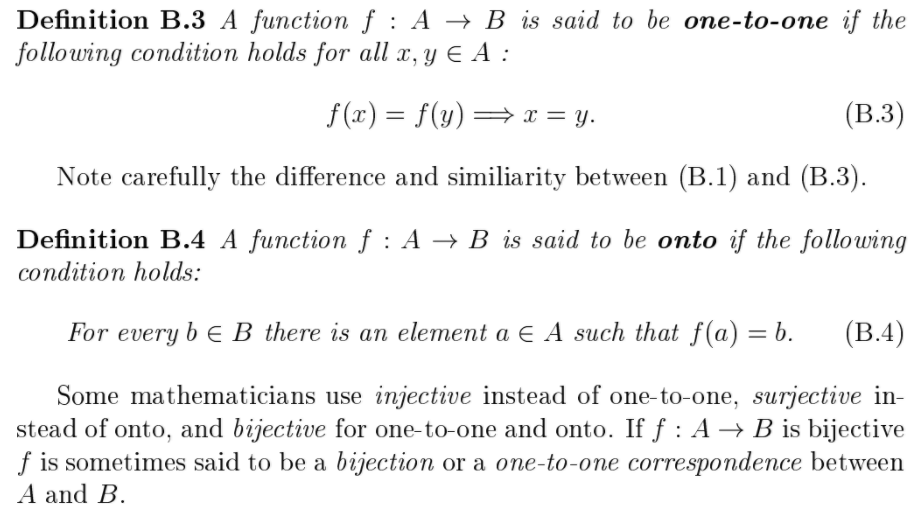
\includegraphics[scale=0.45]{onto}

A function \(f: A \to B\) is said to be \textbf{one-to-one} or \textbf{injective} if the following condition holds for all \(x, y \in A\):

\[
f(x) = f(y) \implies x = y
\]

A function \(f: A \to B\) is said to be \textbf{onto} or \textbf{surjective} if the following condition holds:

\[
\forall \ b \in B \ \exists \ a \in A \ | \ f(a) = b
\]

A function \(f: A \to B\) is said to be \textbf{bijective} if it is both one-to-one and onto. Then \(f\) is sometimes said to be a \textbf{bijection} or a \textbf{one-to-one correspondence} between \(A\) and \(B\).

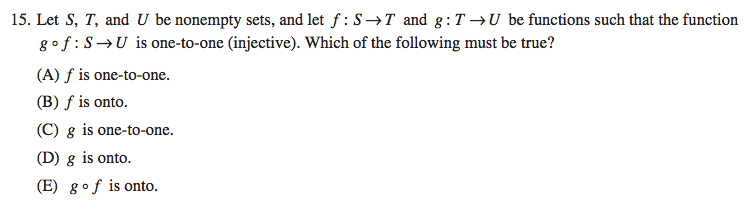
\includegraphics[scale=0.65]{1268_15}

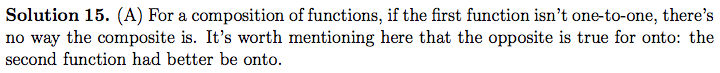
\includegraphics[scale=0.65]{1268_15s}

Let \(S\) be a set. The \textbf{power set} \(\mathcal{P}(S)\) of \(S\) is the set of all subsets of \(S\) (including \(S\) itself).

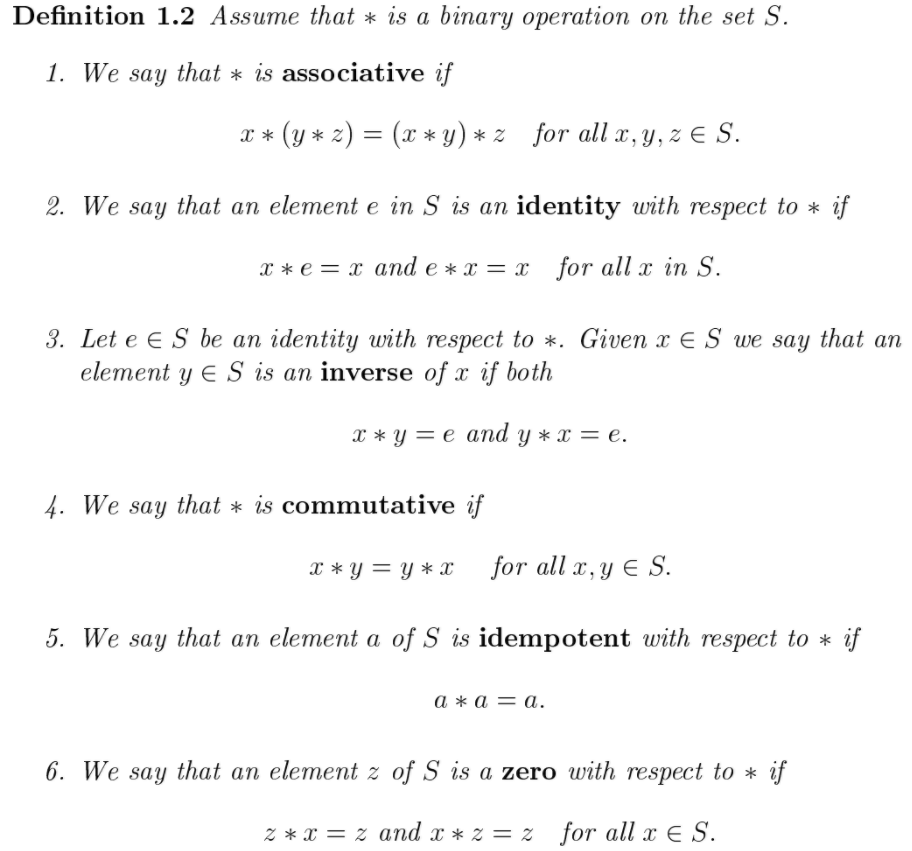
\includegraphics[scale=0.45]{binary_operation2}

\pagebreak

For each integer \(n \geq 2\) define the set

\[
\mathbb{Z}_n = \{0, 1, 2, \ldots, n-1\}
\]

For all \(a, b \in \mathbb{Z}_n\) let \[a + b = \text{remainder when the ordinary sum of a and b is divided by n}\] and \[a \cdot b = \text{remainder when the ordinary product of a and b is divided by n.}\]

These binary operations are referred to as \textbf{addition modulo \(n\)} and \textbf{multiplication modulo \(n\)}. The integer \(n\) in \(\mathbb{Z}_n\) is called the \textbf{modulus}. The plural of modulus is \textbf{moduli}.

Let \(K\) denote any one of the following: \(\mathbb{Z}, \mathbb{Q}, \mathbb{R}, \mathbb{Z}_n\). \[M_n(K)\] is the set of all \(n \times n\) matrices containing elements of \(K\). \[GL(n, K)\] is the set of all matrices in \(M_{n}(K)\) with non-zero determinant. \((GL(n, k), \cdot)\) is called the \textbf{general linear group of degree n over K}. It is non-abelian.

\[
SL(n, K) = \{A \in GL(n, K) \ | \ \det(A) = 1\}
\]

\(SL(n, K)\) is called the \textbf{Special Linear Group of degree \(n\) over \(K\)}.

\pagebreak

% Chapter 2
\section{Chapter 2: Groups}\label{abs.alg.grps.sec}

\begin{definition}\label{abs.alg.group.abelian}

\textbf{Definition} A \textbf{group} is an ordered pair \((G, *)\) where \(G\) is a set and \(*\) is a binary operation on \(G\) satisfying the following properties:

\begin{enumerate}[1.]

\item \textbf{The binary operation is associative on \(G\):} \(\forall \ x, y , z \in G\), 

\[
x * (y * z) = (x * y) * z
\]

\item \textbf{The binary operation contains a (unique) identity in \(G\):} \(\exists \ e \in G \ | \ \forall \ x  \in  G\)

\[
e * x = x, \ x * e = x 
\]

\item \textbf{Every element in \(G\) has a (unique) inverse on \(*\) in \(G\):} \(\forall \ x \in G \ \exists \ y \in G \ |\)

\[
x*y = e, y*x =e
\]

A group \( (G, *)\) is said to be \textbf{abelian} if \(\forall \ x, y \in G, \ x*y = y*x\). A group is said to be \textbf{non-abelian} if it is not abelian.

\end{enumerate}

\end{definition}

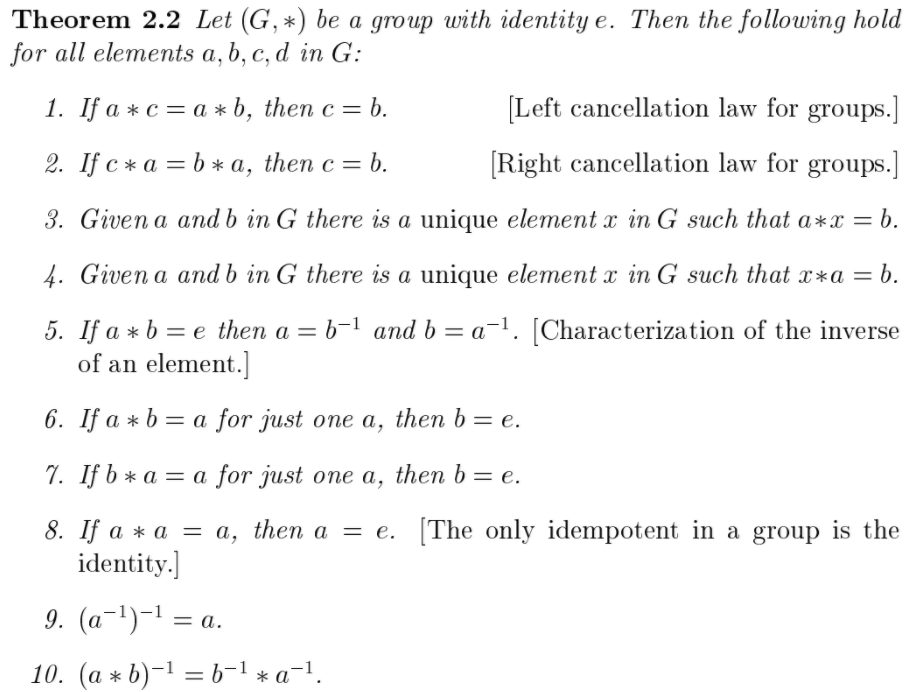
\includegraphics[scale=0.45]{group_properties}

\pagebreak
% Chapter 3
\section{Chapter 3: The Symmetric Groups}\label{abs.alg.sec.sym}

If \(n\) is a positive integer, \[[n] = \{ 1, 2, \ldots, n \} \] A \textbf{permutation} of \([n]\) is a one-to-one, onto function from \([n]\) to \([n]\), and \[S_n\] is the set of all permutations of \([n]\).

The identity of \(S_n\) is the so-called \textbf{identity function}

\[
\iota : [n] \to [n]
\]

which is defined by the rule

\[
\iota(x) = x, \ \ \forall \ x \in [n]
\]

\textbf{The inverse of an element \(\sigma \in S_n\):} Suppose \(\sigma \in S_n\). Since \(\sigma\) is by definition one-to-one and onto, the rule

\[
\sigma^{-1}(y) = x \iff \sigma(x) = y
\]

defines a function \(\sigma^{-1}: [n] \to [n]\). This function \(\sigma^{-1}\) is also one-to-one and onto and satisfies

\[
\sigma \sigma^{-1} = \iota \text{       and         } \sigma^{-1}\sigma = \iota
\]

so it is the inverse of \(\sigma\) in the group sense also.

Since the binary operation of composition on \(S_n\) is associative [\(  (\gamma \beta) \alpha = \gamma (\beta \alpha)  \)], \(S_n\) under the binary operation of composition is a group (it is associative, it has an inverse, and it has an identity).

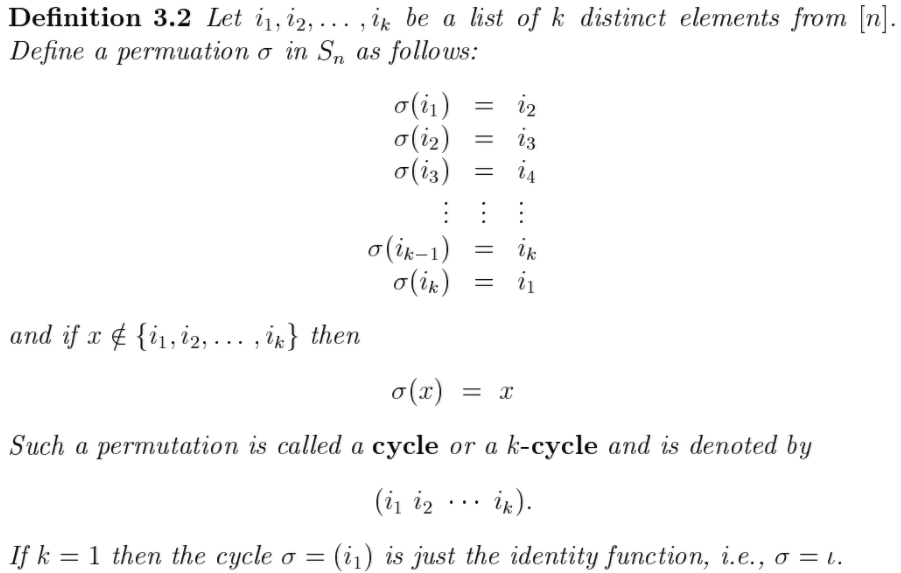
\includegraphics[scale=0.45]{cycle}

Two cycles \((i_1 \ i_2 \ \ldots \ i_k)\) and \((j_1 \ j_2 \ \ldots \ j_l)\) are said to be \textbf{disjoint} if the sets \(\{i_1, i_2, \ldots, i_k\}\) and \(\{j_1, j_2, \ldots, j_l\}\) are disjoint.

So for example, the cycles \((1 \ 2 \ 3)\) and \((4 \ 5 \ 8)\) are disjoint, but the cycles \((1 \ 2 \ 3)\) and \((4 \ 2 \ 8)\) are not disjoint.

If \(\sigma\) and \(\tau\) are disjoint cycles, then \(\sigma \tau = \tau \sigma\).

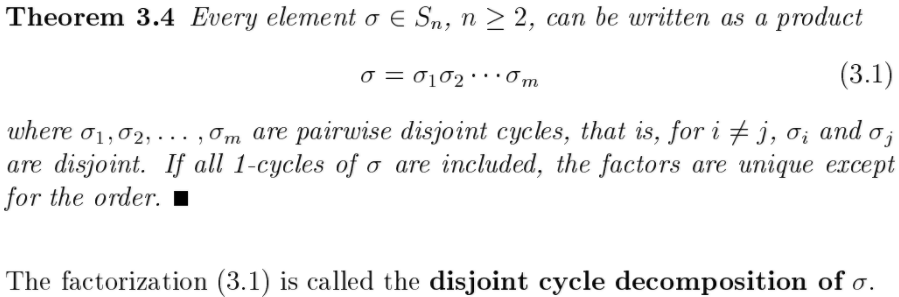
\includegraphics[scale=0.45]{disjoint_cycle_decomp}

An element of \(S_n\) is called a \textbf{transposition} if and only if it is a 2-cycle. 

Every element of \(S_n\) can be written as a product of transpositions. The factors of such a product are not unique. However, if \(\sigma \in S_n\) can be written as a product of \(k\) transpositions and if the same \(\sigma\) can also be written as a product of \(l\) transpositions, then \(k\) and \(l\) have the same parity.

A permutation is \textbf{even} if it is a product of an even number of transpositions and \textbf{odd} if it is a product of an odd number of transpositions. We define the function \(\text{sign} : S_n \to \{1, -1\}\) by 

\[
\text{sign}(\sigma) = \begin{cases} 
     1 & \text{if } \sigma \text{ is even} \\
     -1 & \text{if } \sigma \text{ is odd}
   \end{cases}
\]

If \(n = 1\) then there are no transpositions. In this case, to be complete we define the identity permutation \(\iota\) to be even.

If \(\sigma\) is a \(k\)-cycle, then \(\text{sign}(\sigma) = 1\) if \(k\) is odd and \(\text{sign}(\sigma) = -1\) if \(k\) is even.

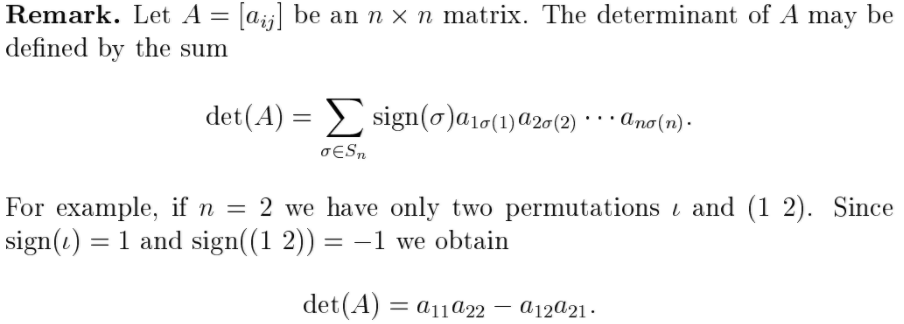
\includegraphics[scale=0.45]{determinant}

\textbf{Definition:} If \((G, *)\) is a group, the number of elements in \(G\) is called the \textbf{order} of \(G\). We use \(|G|\) to denote the order of \(G\). Note that \(|G|\) may be finite or infinite.

Let \[A_n\] be the set of all even permutations in the group \(S_n\). \(A_n\) is called the \textbf{alternating group of degree \(n\)}.

\pagebreak
% Chapter 4
\section{Chapter 4: Subgroups}

\textbf{Definition:} Let \(G\) be a group. A \textbf{subgroup} of \(G\) is a subset \(H\) of \(G\) which satisfies the following three conditions:


\begin{enumerate}[1.]

\item \(e \in H\)

\item \(a, b \in H \implies ab \in H\)

\item \(a \in H \implies a^{-1} \in H\)

\end{enumerate}


If \(H\) is a subgroup of \(G\), we write \(H \leq G\). The subgroups \(\{e\}\) and \(G\) are said to be \textbf{trivial} subgroups of \(G\).

Every finite subgroup may be thought of as a subgroup of one of the groups \(S_n\).

Let \(A_n\) be the set of all even permutations in the group \(S_n\). \(A_n\) is then a subgroup of \(S_n\). \(A_n\) is called the \textbf{alternating group of degree \(n\)}.

Let \(a\) be an element of the group \(G\). If \(\exists \ n \in \mathbb{N} \ | \ a^n = e\) we say that \(a\) has \textbf{finite order} and we define

\[
\text{o}(a) = \min \{n \in \mathbb{N} \ | \ a^n = e\}
\]

If \(a^n \neq e \ \forall \ n \in \mathbb{N}\) we say that \(a\) has \textbf{infinite order} and we define

\[
\text{o}(a) = \infty
\]

In either case we call \(\text{o}(a)\) the \textbf{order} of \(a\). Note carefully the difference between the order of a group and the order of an element of a group. Note also that \(a = e \iff \text{o}(a) = 1\). So every element of a group other than \(e\) has order \(n \geq 2\) or \(\infty\).

Let \(a\) be an element of group \(G\). Define

\[
\langle a \rangle = \{a^i  : i \in \mathbb{Z} \}
\]

We call \(\langle a \rangle\) the \textbf{subgroup of \(G\) generated by \(a\)}. Note that \(e = a^0\) and \(a^{-1}\) are in \(\langle a \rangle\).

\textbf{Theorem.} For each \(a \in G\), \(\langle a \rangle\) is a subgroup of \(G\). \(\langle a \rangle\) contains \(a\) and is the smallest subgroup of \(G\) containing \(a\). 

\textbf{Proof of second statement.} If \(H\) is any subgroup of \(G\) containing \(a\), \(\langle a \rangle \subseteq H \) since \(H\) is closed under taking products and inverses. That is, every subgroup of \(G\) containing \(a\) also contains \(\langle a \rangle\). This implies that \(\langle a \rangle\) is the smallest subgroup of \(G\) containing \(a\).

\pagebreak 
\textbf{Theorem.} Let \(G\) be a group and let \(a \in G\). If \(\text{o}(a) = 1\), then \(\langle a \rangle = \{e \}\). If \(\text{o}(a) = n\) where \(n \geq 2\), then

\[
\langle a \rangle = \{e, a, a^2, \ldots, a^{n-1} \}
\]

and the elements \(e, a, a^2, \ldots, a^{n-1}\) are distinct; that is, 

\[
\text{o}(a) = | \langle a \rangle |
\]

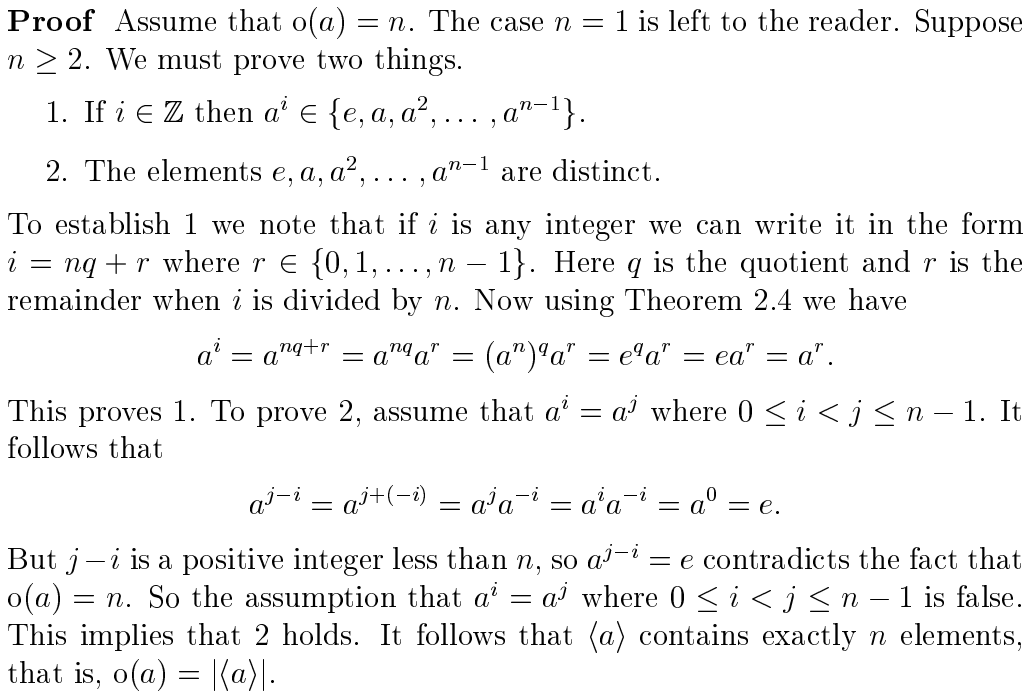
\includegraphics[scale=0.4]{ch4_proof}

\textbf{Theorem.} If \(G\) is a finite group, then every element of \(G\) has finite order.

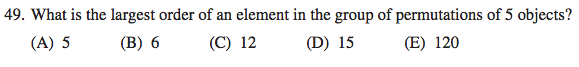
\includegraphics[scale=0.65]{1268_49}

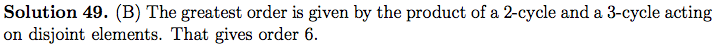
\includegraphics[scale=0.65]{1268_49s}

\pagebreak
% Chapter 5
\section{Chapter 5: The Group of Units of \(\mathbb{Z}_n\)}

Let \(n \geq 2\). An element \(a \in \mathbb{Z}_n\) is said to be a \textbf{unit} if \(\exists \ b \in \mathbb{Z}_n \ | \ ab = 1\) (where the product is multiplication modulo \(n\)). 

The set of all units in \(\mathbb{Z}_n\) is denoted by \[U_n\] and is a group under multiplication modulo \(n\) called the \textbf{group of units of \(\mathbb{Z}_n\)}.

\textbf{Theorem.} For \(n \geq 2 \), \(U_n = \{a \in \mathbb{Z}_n: \gcd(a, n) = 1 \} \)

\textbf{Theorem.} \(p\) is a prime \(\implies \exists \ a \in U_p \ | \ U_p = \langle a \rangle\)

\textbf{Theorem.} If \(n \geq 2\) then \(U_n\) contains an element \(a\) satisfying \(U_n = \langle a \rangle\) if and only if \(a\) has one of the following forms: \(2, \ 4, \ p^k\), or \(2p^k\) where \(p\) is an odd prime and \(k \in \mathbb{N}\).

%\pagebreak
% Chapter 6
\section{Chapter 6: Direct Products of Groups}

If \(G_1, G_2, \ldots, G_n\) is a list of \(n\) groups we make the Cartesian product \(G_1 \times G_2 \times \cdots \times G_n\) into a group by defining the binary operation

\[
(a_1, a_2, \ldots, a_n) \cdot (b_1, b_2, \ldots, b_n) = (a_1 \cdot b_1, a_2 \cdot b_2, \ldots, a_n \cdot b_n)
\]

Here for each \(i \in \{1, 2, \ldots, n\}\) the product \(a_i \cdot b_i\) is the product of \(a_i\) and \(b_i\) in the group \(G_i\). We call this group the \textbf{direct product} of the groups \(G_1, G_2, \ldots, G_n\).

The direct product contains an identity and an inverse, and is associative (since it is composed of groups which must themselves be associative), so it is a group per below:

\textbf{Theorem.} If \(G_1, G_2, \ldots, G_n\) is a list of \(n\) groups, the direct product \(G = G_1 \times G_2 \times \cdots \times G_n\) as defined above is a group. Moreover, if for each \(i\), \(e_i\) is the identity of \(G_i\), then \(e_1, e_2, \ldots, e_n\) is the identity of \(G\), and if 

\[
\boldsymbol{a} = (a_1, a_2, \ldots, a_n) \in G
\]

then the inverse of \(\boldsymbol{a}\) is given by

\[
\boldsymbol{a}^{-1} = (a_1^{-1}, a_2^{-1}, \ldots, a_n^{-1})
\]

where \(a_i^{-1}\) is the inverse of \(a_i\) in the group \(G_i\).

\pagebreak
% Chapter 7
\section{Chapter 7: Isomorphism of Groups}

Let \(G = \{g_1, g_2, \ldots, g_n \}\). Let \(\text{o}(g_i) = k_i\) for \(i = 1, 2 , \ldots, n\). We say that the sequence \((k_1, k_2, \ldots, k_m) \) is the \textbf{order sequence} of the group \(G\). To make the sequence unique we assume the elements are ordered so that \(k_1 \leq k_2 \leq \ldots \leq k_n\).

Let \((G, *)\) and \((H, \bullet)\)  be groups. A function \(f : G \to H\) is said to be a \textbf{homomorphism} from \(G\) to \(H\) if

\[
f(a * b) = f(a) \bullet f(b)
\]

for all \(a, b \in G\). If in addition \(f\) is one-to-one and onto, \(f\) is said to be an \textbf{isomorphism} from \(G\) to \(H\).

We say that \(G\) and \(H\) are \textbf{isomorphic} if and only if there is an isomorphism from \(G\) to \(H\). We write \(G \cong H\) to indicate that \(G\) is isomorphic to \(H\).

\textbf{Isomorphism is an equivalence relation:} If \(G, H\), and \(K\) are groups then

\begin{enumerate}[1.]

\item \(G \cong G\)

\item If \(G \cong H\) then \(H \cong G\), and

\item If \(G \cong H\) and \(H \cong K\), then \(G \cong K\).

\end{enumerate}

\textbf{Theorem.} Let \((G, *)\) and \((H, \bullet)\) be groups and let \(f: G \to H\) be a homomorphism. Let \(e_G\) denote the identity of \(G\), and let \(e_H\) denote the identity of \(H\). Then

\begin{enumerate}[1.]

\item \(f(e_G) = e_H\)

\begin{center}
\textit{Proof: Let \(x_G \in G\) and let \(f(x_G) = x_H \in H\). Then \(x_H = f(x_G) = f(e_G * x_G) = f(e_G) \bullet f(x_G) = f(e_G) \bullet x_H = e_H \bullet x_H\).}
\end{center}

\item \(f(a^{-1}) = f(a)^{-1}\)

\begin{center}
\textit{Proof: \(f(a)^{-1} \bullet f(a) = e_H = f(e_G) = f(a^{-1} * a) = f(a^{-1}) \bullet f(a)\)}
\end{center}

\item \(f(a^n) = f(a)^n \ \forall \ n \in \mathbb{Z}\)

\begin{center}
\textit{Proof by induction.}
\end{center}

\end{enumerate}

\textbf{Theorem.} Let \((G, *)\) and \((H, \bullet)\) be groups and let \(f:G \to H\) be an isomorphism. Then \(\text{o}(a) = \text{o}(f(a)) \ \forall \ a \in G\). It follows that \(G\) and \(H\) have the same number of elements of each possible order.

\textbf{Theorem.} If \(G\) and \(H\) are isomorphic groups, and \(G\) is abelian, then so is \(H\).

\begin{center}
\textit{Proof: Let \(a_G, b_G \in G\) and let \(f(a_G) = a_H \in H, f(b_G) = b_H \in H\). \(a_H \bullet b_H = f(a_G) \bullet f(b_G) = f(a_G * b_G) = f(b_G * a_G) = f(b_G) \bullet f(a_G) = b_H \bullet a_H\).}
\end{center}

\begin{definition}[\textbf{Cyclic groups and generators}]\label{abs.alg.def.generator}

A group \(G\) is \textbf{cyclic} if there is an element \(a \in G \ | \ \langle a \rangle = G\). If \(\langle a \rangle = G\) then we say that \(a\) is a \textbf{generator} for \(G\). 

\end{definition}

\textbf{Theorem.} If \(G\) and \(H\) are isomorphic groups and \(G\) is cyclic then \(H\) is cyclic.

\textbf{Theorem.} Let \(a\) be an element of group \(G\). 

\begin{enumerate}[1.]

\item \(\text{o}(a) = \infty \implies \langle a \rangle \cong \mathbb{Z}\).

\item \(\text{o}(a) = n \in \mathbb{N} \implies \langle a \rangle \cong \mathbb{Z}_n\)

\end{enumerate}

%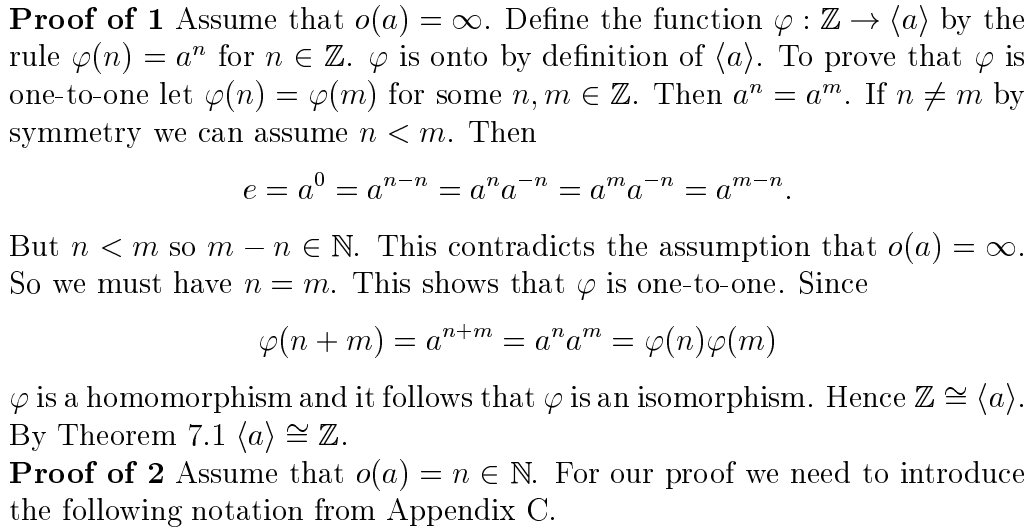
\includegraphics[scale=0.4]{cyclic_order_proof1}

%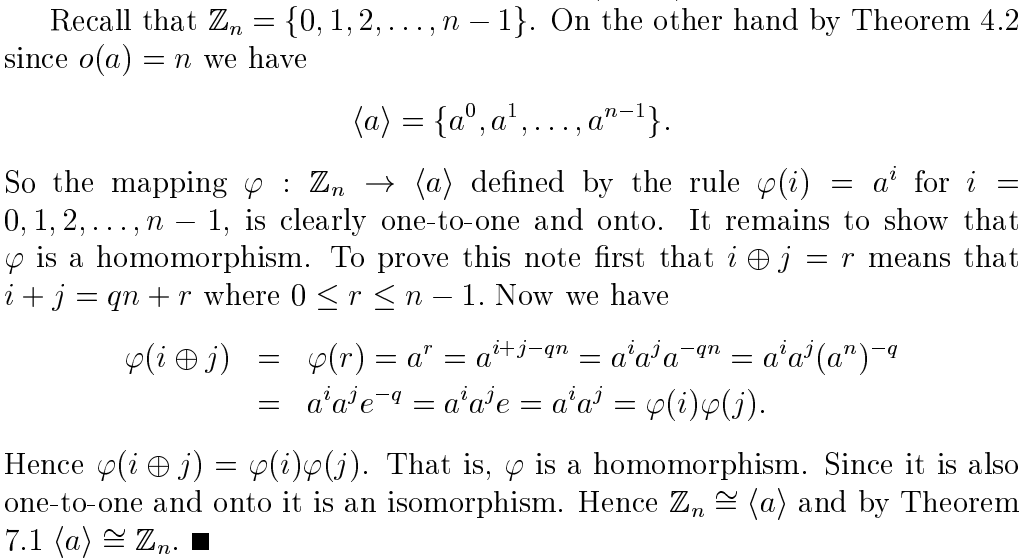
\includegraphics[scale=0.4]{cyclic_order_proof2}

\textbf{Cayley's Theorem.} If \(G\) is a finite group of order \(n\), then there is a subgroup \(H\) of \(S_n\) such that \(G \cong H\).

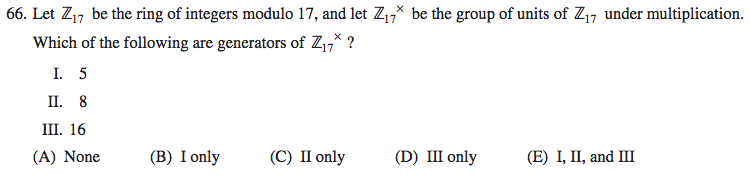
\includegraphics[scale=0.65]{1268_66}

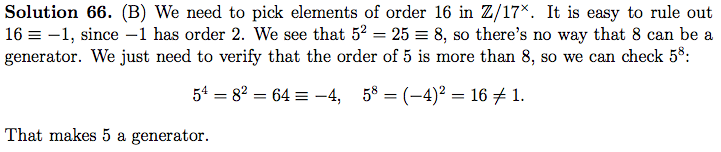
\includegraphics[scale=0.65]{1268_66s}

\pagebreak
% Chapter 8
\section{Chapter 8: Cosets and Lagrange's Theorem}

Let \(G\) be a group and let \(H\) be subgroup of \(G\). For each element \(a\) of \(G\) we define

\[
aH = \{ ah \ | \ h \in H\}
\]

We call \(aH\) the \textbf{coset of \(H\) in \(G\) generated by \(a\)}.

Let \(a, b \in G\). Then

\begin{enumerate}[1.]

\item \(a \in aH\) (since \(H\) must contain an identity; specifically, the identity of \(G\))

\item \(|aH| = |H|\) (since \(ah\) is unique)

\item \(aH \cap bH \neq  \emptyset \implies aH = bH\)

\end{enumerate}

\textbf{Lagrange's Theorem.} If \(G\) is a finite group and \(H \leq G\) then \(|H|\) divides \(|G|\).

Any group of prime order is cyclic; therefore, there is only one such group up to isomorphism.

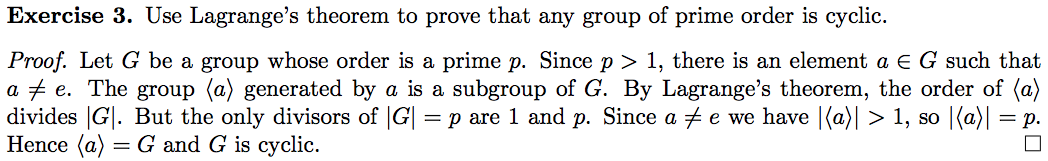
\includegraphics[scale=0.45]{prime_order}

We say that there are \(k\) \textbf{isomorphism classes of groups of order \(n\)} if there are \(k\) groups \(G_1, G_2, \ldots, G_k\) such that

\begin{enumerate}[1.]

\item if \(i \neq j\) then \(G_i\) and \(G_j\) are not isomorphic, and

\item Every group of order \(n\) is isomorphic to \(G_i\) for some \(i \in \{1, 2, \ldots, k\}\).

\end{enumerate}

This is sometimes expressed by saying that "there are \(k\) groups of order \(n\) up to isomorphism" or that "there are \(k\) non-isomorphic groups of order \(n\)."

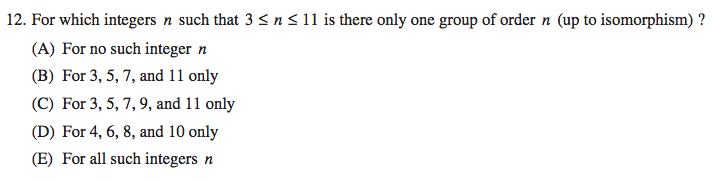
\includegraphics[scale=0.65]{1268_12}

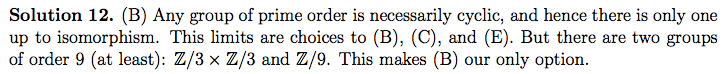
\includegraphics[scale=0.65]{1268_12s}

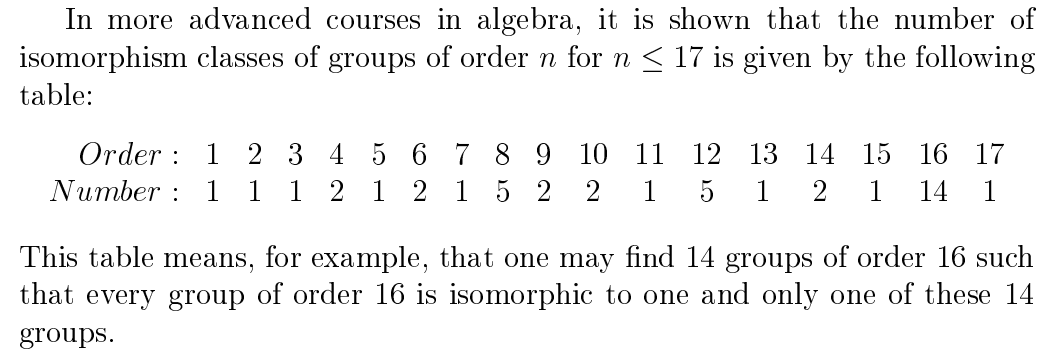
\includegraphics[scale=0.45]{isomorphism_groups_order}

There is only one isomorphism class of groups of order \(n\) if \(n\) is prime. But there are some non-primes that have this property; for example, 15.

\textbf{The Fundamental Theorem of Finite Abelian Groups.} If \(G\) is a finite abelian group of order at least 2, then 

\[
G \cong \mathbb{Z}_{p_1^{n_1}} \times \mathbb{Z}_{p_2^{n_2}} \times \cdots \times \mathbb{Z}_{p_s^{n_s}} 
\]

where for each \(i\), \(p_i\) is a prime and \(n_i\) is a positive integer. Moreover, the prime powers \(p_i^{n_i}\) are unique except for the order of the factors.

If the group \(G\) in the above theorem has order \(n\) then

\[
n = p_1^{n_1}p_2^{n_2} \cdots p_s^{n_2}
\]

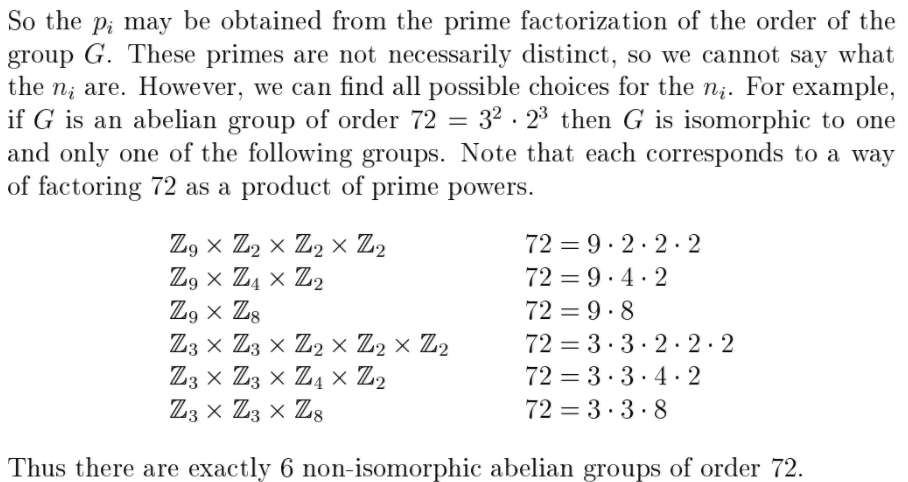
\includegraphics[scale=0.45]{isomorphism_groups_order2}

\textbf{Corollary.} For \(n \geq 2\), the number of isomorphism classes of abelian groups of order \(n\) is equal to the number of ways to factor \(n\) as a product of prime powers (where the order of the factors does not count).

%\textbf{Remark:} In number theory it is proven that if \(n = ab\) and \(\gcd(a, b) = 1\) then \(\mathbb{Z}_n \cong \mathbb{Z_a} \times \mathbb{Z_b}\). This is called the \textit{Chinese Remainder Theorem.}

\pagebreak
% Chapter 9
\section{Chapter 9: Introduction to Ring Theory}\label{abs.alg.sec.ring}

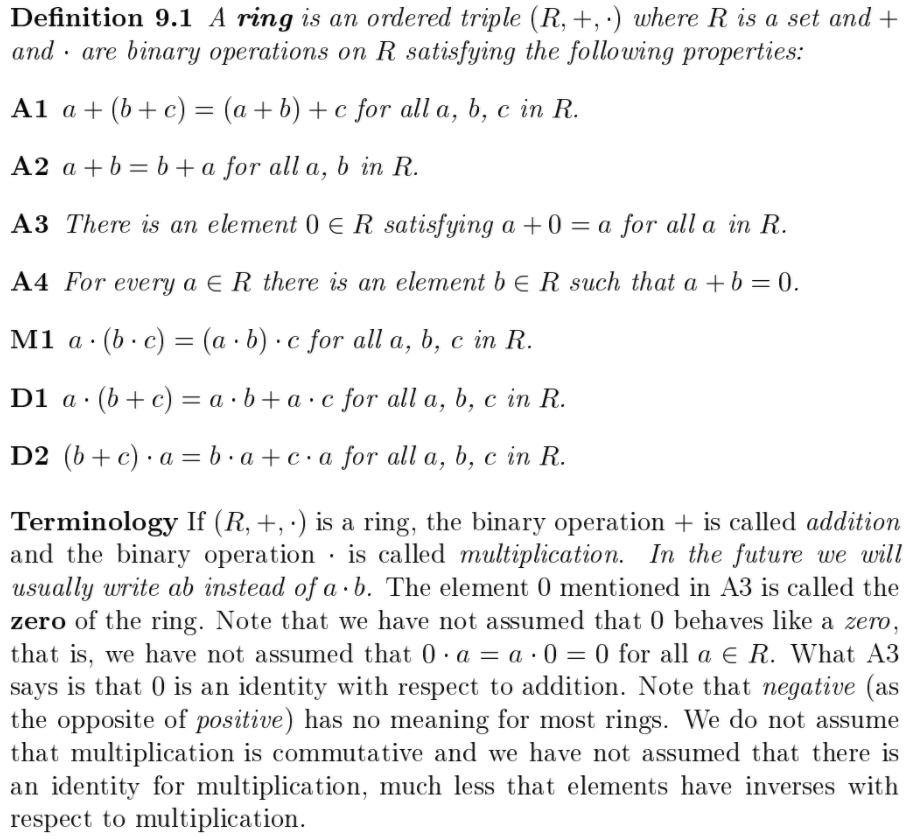
\includegraphics[scale=0.45]{ring_summary}

\begin{definition}[\textbf{Ring; definition from Section 2.1 of \citet{lang2005algebra}, p. 98 of pdf, p. 83 of book)}]\label{abs.alg.def.ring}

A \textbf{ring} \(A\) is a set, together with two laws of composition called multiplication and addition respectively, and written as a product and as a sum respectively, satisfy the following conditions:

\begin{enumerate}


\item With respect to addition, \(A\) is a commutative group.

\item The multiplication is associative, and has a unit element.

\item For all \(x,y, z \in A\), we have \((x+y)z = xz + yz\) and \(z(x+y) = zx + zy\). (This is called \textbf{distributivity}.

\end{enumerate}

As usual, we denote the unit element for addition by 0, and the unit element for multiplication by 1. We do not assume that \(1 \neq 0\). 

\end{definition}

\begin{definition}

Let \(A\) be a ring, and let \(U\) be the set of elements of \(A\) which have both right and left inverse. Then \(U\) is a multiplicative group. Indeed, if \(a\) has a right inverse \(b\), so that \(ab = 1\), and a left inverse \(c\), so that \(ca=1\), then \(c = cab= b\), so \(c=b\), and we see that \(c\) (or \(b\)) is a two-sided inverse, and that \(c\) itself has a two-sided inverse, namely \(a\). Therefore \(U\) satisfies all the axioms of a multiplicative group, and is called the group of \textbf{units} of \(A\). It is sometimes denoted by \(A^*\), and is also called the group of \textbf{invertible} elements of \(A\). A ring \(A\) such that \(1 \neq 0\) and such that every non-zero element is invertible is called a \textbf{division ring}.

\end{definition}


\begin{definition}

A ring \(A\) is said to be \textbf{commutative} if \(xy = yx\) for all \(x, y \in A\). A commutative division ring is called a \textbf{field}. We observe that by definition, a field contains at least two elements, namely 0 and 1. 

\end{definition}

\begin{definition}

A subset \(B\) of a ring \(A\) is called a \textbf{subring} if it is an additive subgroup, if it contains the multiplicative unit, and if \(x, y \in B\) implies \(xy \in B\). If that is the case, then \(B\) itself is a ring, the laws of operation in \(B\) being the same as the laws of operation in \(A\).

For example, the \textbf{center} of a ring \(A\) is the subset \(A\) consisting of all elements of \(a \in A\) such that \(ax = xa\) for all \(x \in A\). (One sees immediately that the center of \(A\) is a subring.)

\end{definition}

\begin{definition}[\textbf{Ideal; definition from Section 2.1 of \citet{lang2005algebra}, p. 101 of pdf, p. 86 of book)}]\label{abs.alg.def.ring.ideal}

A \textbf{left ideal} \(a\) in a ring \(A\) is a subset of \(A\) which is a subgroup of the additive group of \(A\), such that \(A a \subset a\) (and hence \(Aa = a\) since \(A\) contains 1). To define a right ideal, we require \(aA = a\), and a \textbf{two-sided ideal} is a subset which is both a left and a right ideal. A two-sided ideal is called simply an \textbf{ideal}. Note that \((0)\) and \(A\) itself are ideals.

\end{definition}

\begin{definition}[\textbf{Generator; definition from Section 2.1 of \citet{lang2005algebra}, p. 101 of pdf, p. 86 of book)}]\label{abs.alg.def.ring.generator}

If \(A\) is a ring and \(a \in A\), then \(Aa\) is a left ideal, called \textbf{principal}. We say that \(a\) is a generator of \(a\) (over \(A\)). Similarly, \(AaA\) is a principal two-sided ideal of we define \(AaA\) to be the set of all sums \(\sum x_i a y_i\) with \(x_i, y_i \in A\). More generally, let \(a_1, \ldots, a_n\) be elements of \(A\). We denote by \((a_1, \ldots, a_n)\) the set of elements of \(A\) which can be written in the form

\[
x_1 a_1 + \ldots + x_n a_n, \qquad x_i \in A.
\]

Then this set of elements is immediately verified to be a left ideal, and \(a_1, \ldots, a_n\) are called \textbf{generators} of the left ideal. 

See also Definition \ref{abs.alg.def.generator}.

\end{definition}

If \(\{a_i\}_{i \in I}\) is a family of ideals, then their intersection \(\bigcap_{i \in I} a_i\) is also an ideal. Similarly for left ideals. It is easy to verify that if \(a = (a_1, \ldots, a_n)\) then \(a\) is the intersection of all left ideals containing the elements \(a_1, \ldots, a_n\).

\begin{definition}

A ring \(A\) is said to be \textbf{commutative} if \(xy = yx\) for all \(x, y \in A\). In that case, every left or right ideal is two-sided. A commutative ring such that every ideal is principal and such that \(1  \neq 0\) is called a \textbf{principal} ring.

\end{definition}

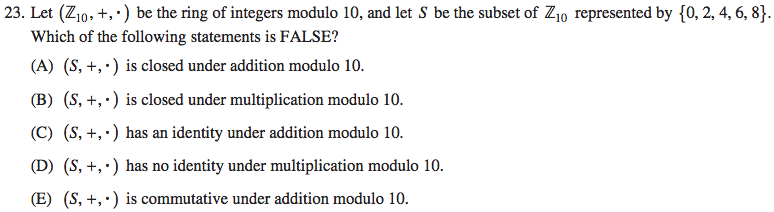
\includegraphics[scale=0.65]{1268_23}

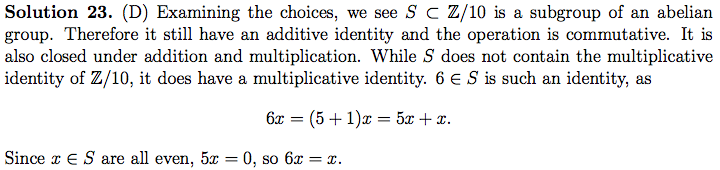
\includegraphics[scale=0.65]{1268_23s}

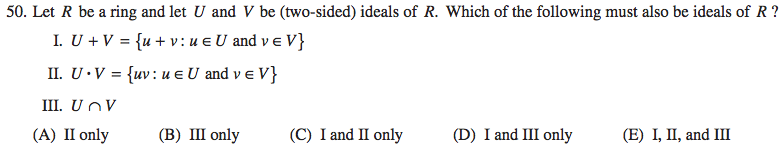
\includegraphics[scale=0.65]{1268_50}

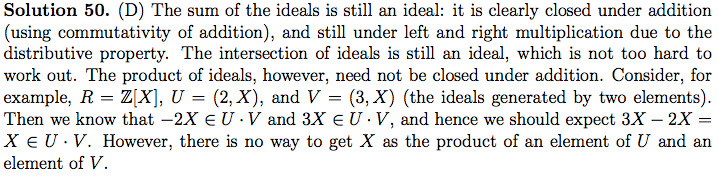
\includegraphics[scale=0.65]{1268_50s}

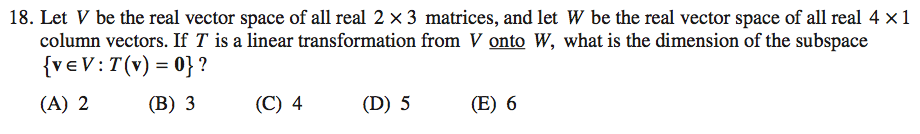
\includegraphics[scale=0.5]{0568_18}

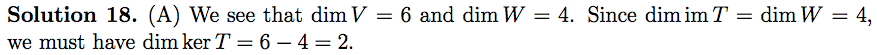
\includegraphics[scale=0.5]{0568_18s}

%\bibliographystyle{abbrvnat}
%\bibliography{mybib2fin}
%
%\end{document}